\newpage
\section{Preliminary Testing}
\subsection{Reason for Experiment}
Before any analysis of the data was done, work was carried out to ensure Calpy behaved as expected and any bugs or potential problems were fixed or documented early. These experiments were designed to measure the effectiveness of the Calpy software using controlled speech where each pause can be counted visually looking at the waveform and artificially constructed precisely using the Audacity software. Then finally testing the software on sample audio files to see what can be expected from the varied chosen datasets. \\

The significance of these tests show the level online systems can be used before being adversely impacted by quality due to noise or compression. In order to build a functioning and useful online system, knowing the limits and strengths of the audio quality can be a major factor in subsequent build requirements. If files require high quality then bandwidth must be high in order for the system to produce meaningful results. This can also affect the equipment used, if a simple inexpensive microphone is used it may place a high cost on the quality of the results due to the amount of compression and information lost through recording to lower quality. This can also affect the environments this can be used in and the placement of recording devices. \\  

\subsubsection{Goals}
\paragraph{1.} Make sure all pauses that are produced are accounted for (not focussing on length, just presence detection)
\paragraph{2.} Make sure all pauses of arbitrary length X are measured correctly by the digital signal processing module and saved accordingly 
\paragraph{3.} See what the difference in quality is like between the two datasets \\

The first two goals ensures that the software is able to extract all pauses distinctly and correctly (in terms of time) for measurement and making inferences from while the third allows for a quick comparison before moving too far forward with the chosen data sets. \\

\subsection{Audacity Testing Overview} 
Real speech was recorded in a quiet environment to make sure no external 
noise was present that could change the outcome. Waveforms were given initial 
stilted dialogue that progressed into more natural and 
relaxed readings of greater time lengths. Pauses were injected into the speech to see that
 it accurately picks up changes in speech in finer grained, controlled levels. 
Finally high fidelity ABC interviews were digitised and analysed to return a benchmark 
of what can be expected from ideal conditions. \\ 

This could be shown in a pause code plot as well to verify the outcomes visually from the 
audio to the analysed Calpy pause code plot, however not all audio files that are used come
in the proper two channel format which pause code requires to distinguish one voice from another.  \\

%The experiments showed Calpy worked as expected bar one exception, Calpy doesn't signal the last pause in the file, meaning any trailing pauses are ignored. 
Almost all pauses were detected correctly and accurately. 
However, the times of the pauses in between words were measured out exactly and distinctly to make 
sure Calpy could pick up the length of each pause. An example of a synthetic audio file is shown in Figure 5.15. \\

Although more tests could be done in this area to further test Calpy's capabilities and 
where it breaks down in terms of rising and falling of voice (thus where pauses are 
determined), these tests showed that Calpy provided enough accuracy to detect the pauses 
and correctly measure all of them from the sample audio files presented, thus allowing for initial tests to commence. \\

\begin{figure}[htbp]
	\centerline{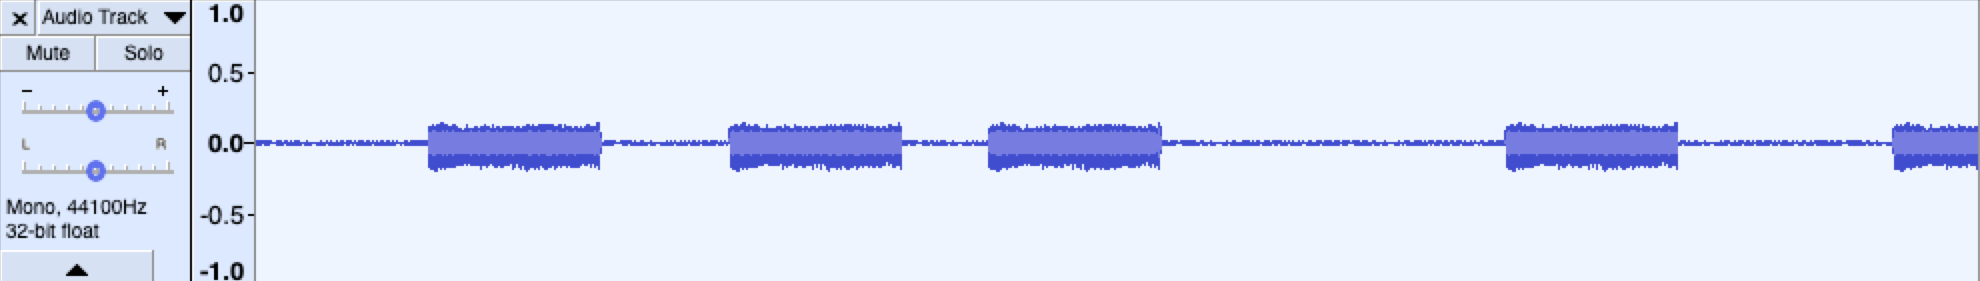
\includegraphics[scale=0.3]{src/main-matter/methodology/preliminary-testing/4170/022}}
	\caption{Example audio file of controlled synthetic utterance and pauses. Each silence is measured out precisely using Audacity}
	\label{flr1}
\end{figure}


\subsection{File format \& frequency}
Mp3 and wav file format were tested, along with the corresponding frequencies from 8000 to 96000 (but only for wav). Testing showed the Calpy software will only accept wav files and not necessarily all wav files either. The original wav audio files had to be converted through audacity first before being digitised, the specific reason was never found. File frequency didn't seem to matter though as Calpy was able to accept anything from 8000+ (this simply increased digitisation time). 
%Knowing how to run Calpy and use wav files correctly took significant troubleshooting. 

\subsubsection{Talkbank}
The Talkbank files could be downloaded in either wav or mp3, however the audio processing library of Calpy does not accept mp3. The wav files were downloaded and transformed through Audacity, taking the mp3 and converting to wav through Audacity to see if this made any difference to results was never tried. The files were available in stereo and could be digitised in either stereo or mono (after transformation through Audacity). 

\subsubsection{Podcasts}
The ABC and JJJ podcasts were available in a high quality wav format. The conditions were in a sound proof room with high quality recording equipment with 2 speakers. These files were really only available in mono, although some files had two channels present when loaded into Audacity the significant overlap of speakers on both channels meant they were effectively mono. Audio files had to be given to Audacity and exported as a wav file with the same file frequency in order for Calpy to accept these files. The right libraries must be imported to handle wav files. Specifically requiring:
\begin{verbatim}
#importing wav
from pydub import AudioSegment #required a brew install ffmpeg
\end{verbatim}

%This was crucial and work could not be done without this installation (this also took significant troubleshooting). 

\subsubsection{Pause Code Plots}
Pause code plots required true stereo so that the file chosen can be split into two channels where each speaker is only in their own channel (i.e. you cant hear the second speaker in the first channel and vice versa). This made the Talkbank files useful for producing the pause code plots. If speaker overlap is present, this will produce a sounding pattern plot that looks like figure 5.16 instead of figure 5.17. \\

Mono audio can't be split into two stereo channels either (channel A with a silent channel B will work, but channel B with a silent channel A will not, not sure why), it must be a stereo split into two mono's. However, significant problems showed up in the pause code when analysed microscopically. The timing of files and their pauses did not match up to the wave form, and some files showed repeated pauses where silence occurred for that speaker (indicating noise present, other speaker was present, or potentially the timing was incorrect for the pause code time stamps). This wasn't investigated further as it wasn't crucial for the investigation (more than likely due to poor audio quality of Talkbank). Examples of incorrect and correct results can be seen below. \\  

\begin{figure}[h!]
	\centerline{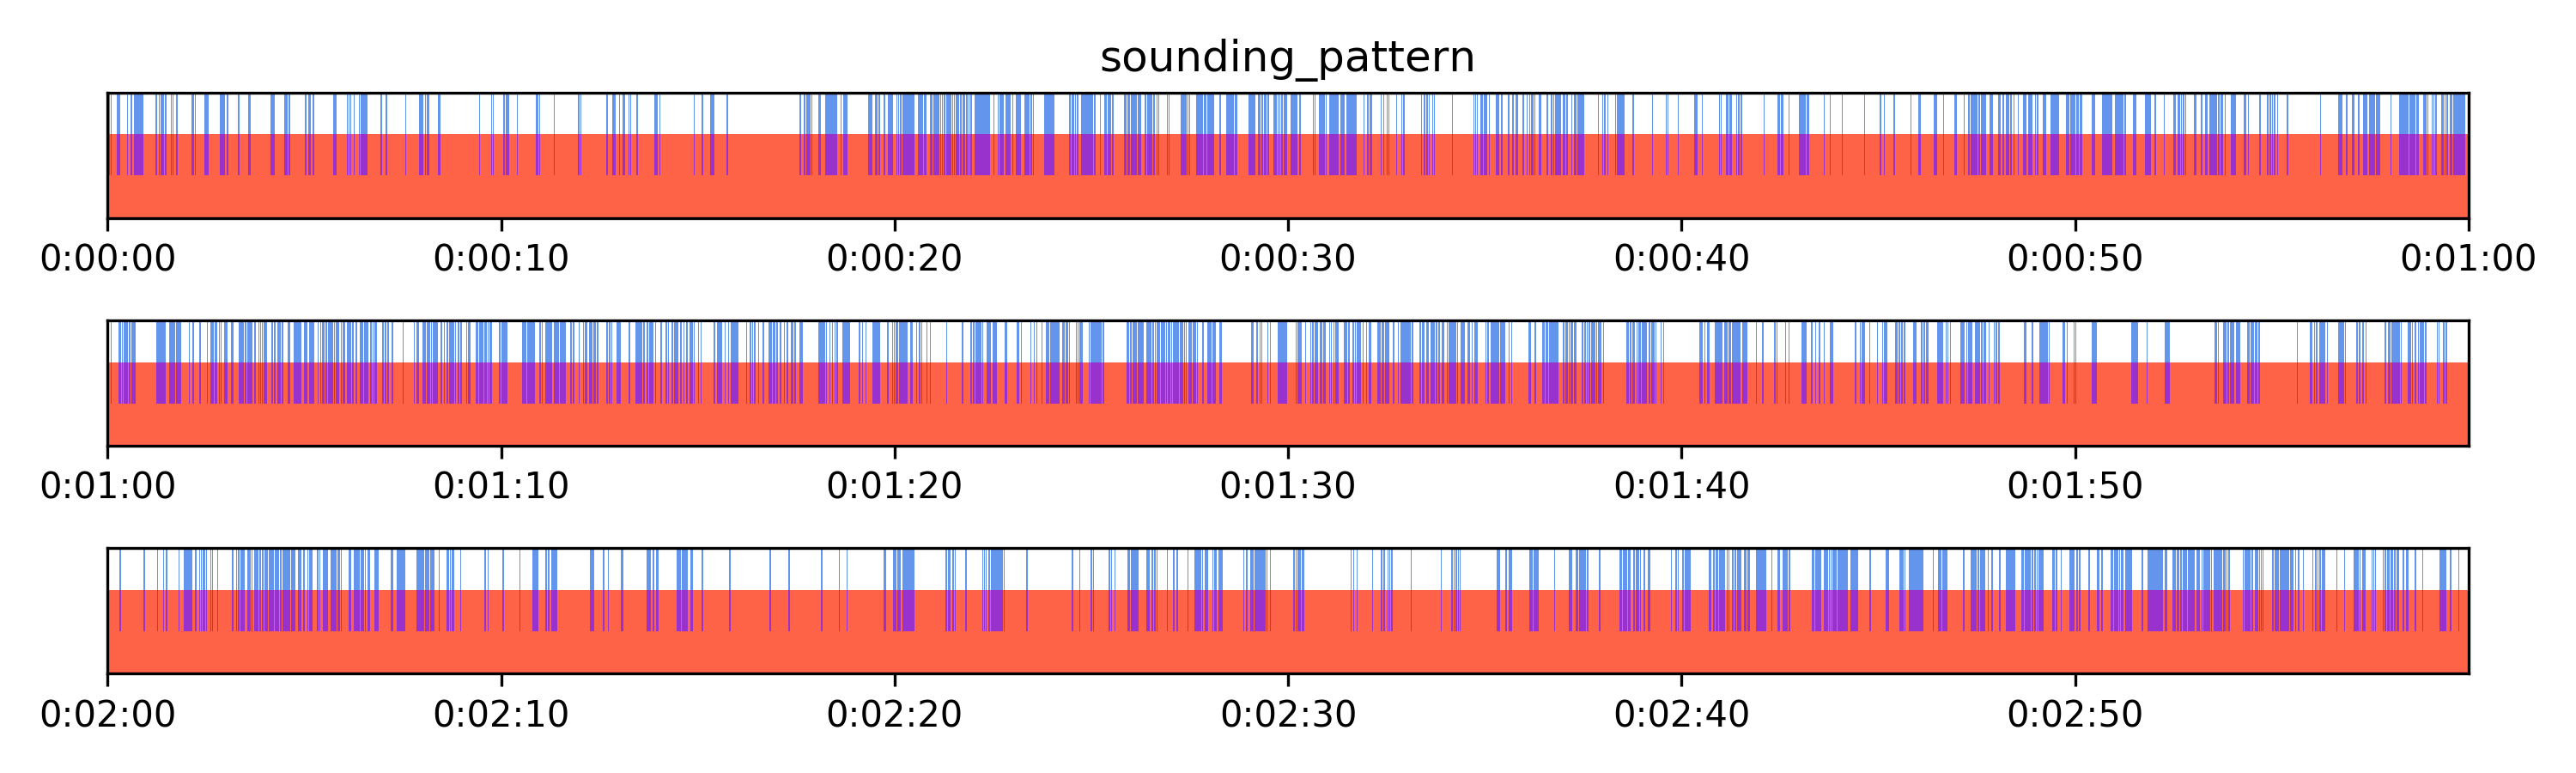
\includegraphics[scale=0.5]{src/main-matter/methodology/preliminary-testing/4170/sounding_pattern_plot_4170_stereo_split}}

	\caption{Entire 4170 - Pause Code Plot - Channel A in blue - Channel B in red. Sounding plot with improper file formatting shows an extended utterance for channel B when no sound exists for that Channel.}
	\label{fig:overlap-sounding}
\end{figure}

\begin{figure}[h!]
	\centerline{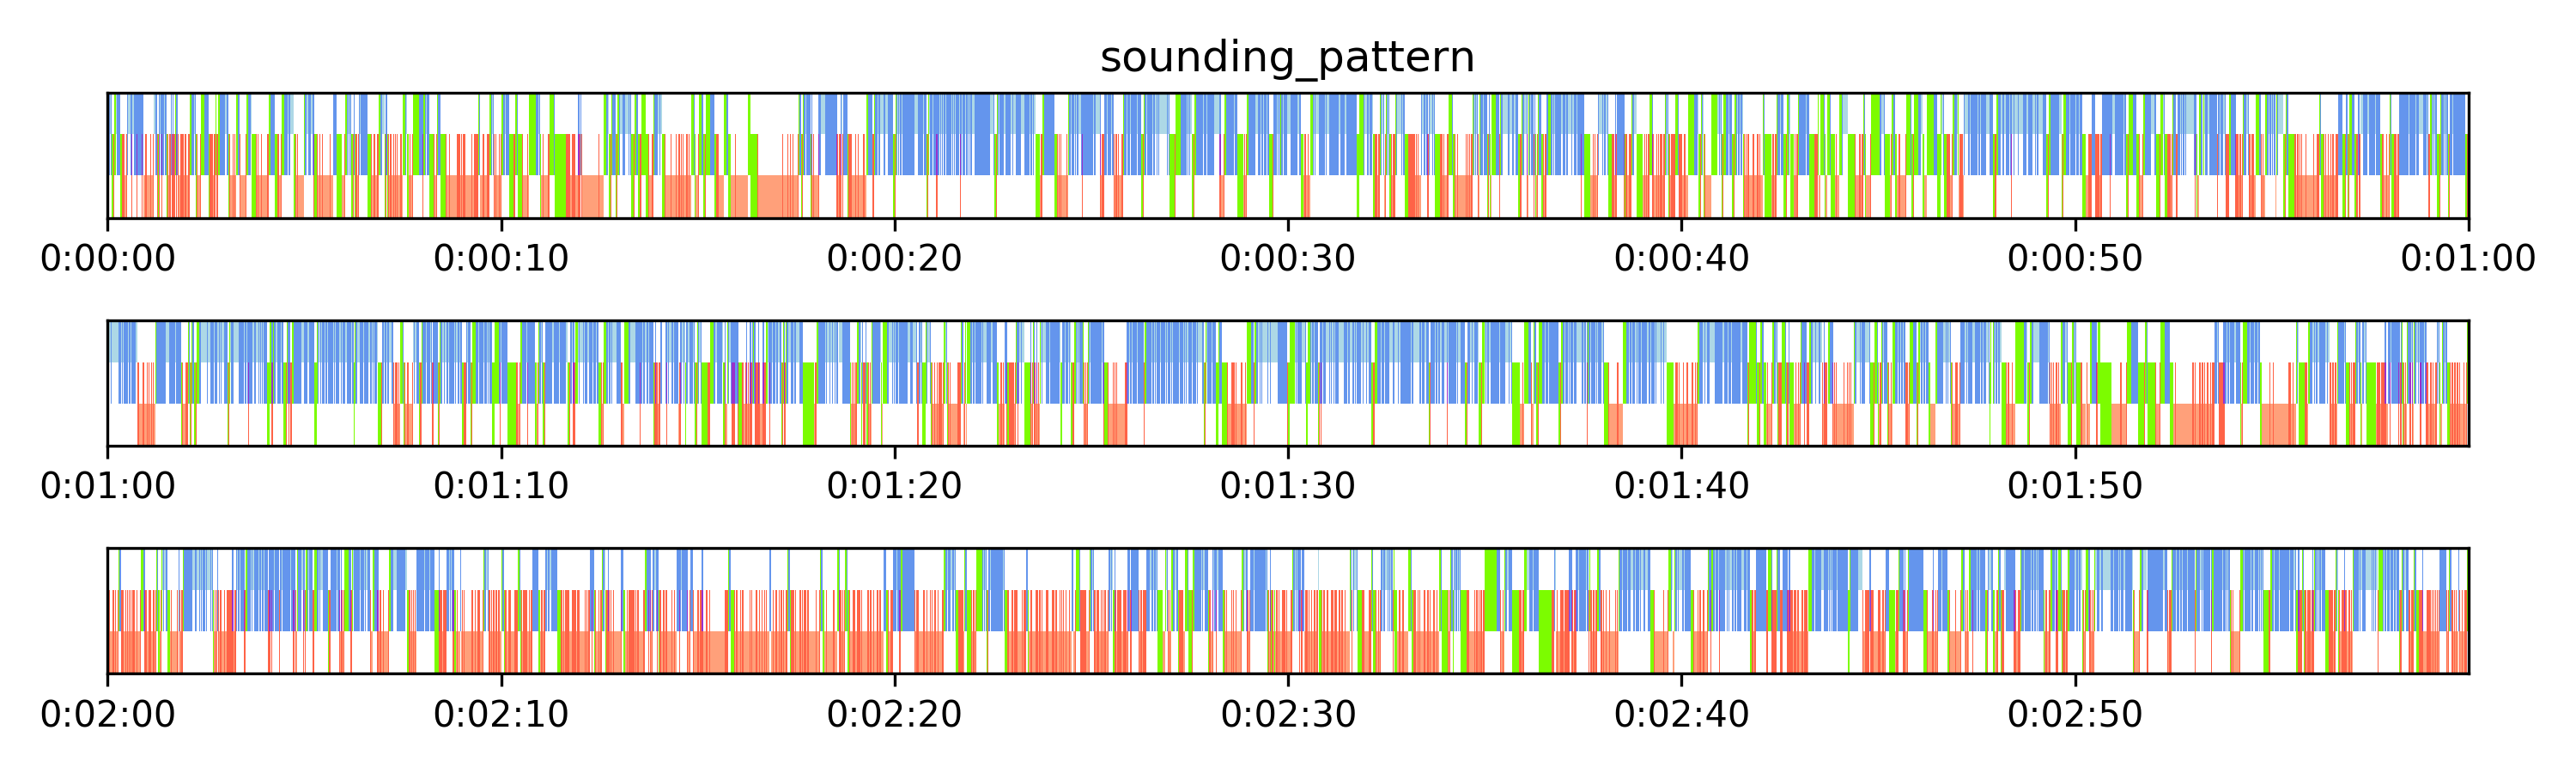
\includegraphics[scale=0.5]{src/main-matter/methodology/preliminary-testing/4170/sounding_pattern_plot_4170_mono_split}}

	\caption{Entire 4170 file - Pause Code Plot - Channel A in blue - Channel B in red. Sounding plot with proper file formatting where both channels are correctly separated and contain different audio tracks.}
	\label{fig:separate-sounding}
\end{figure}

An example of pause code producing incorrect results for two waveforms can be seen in Figures 5.18-21. The wave form shows no audio present for channel B yet utterance can be seen. 

\begin{figure}[h!]
	\centerline{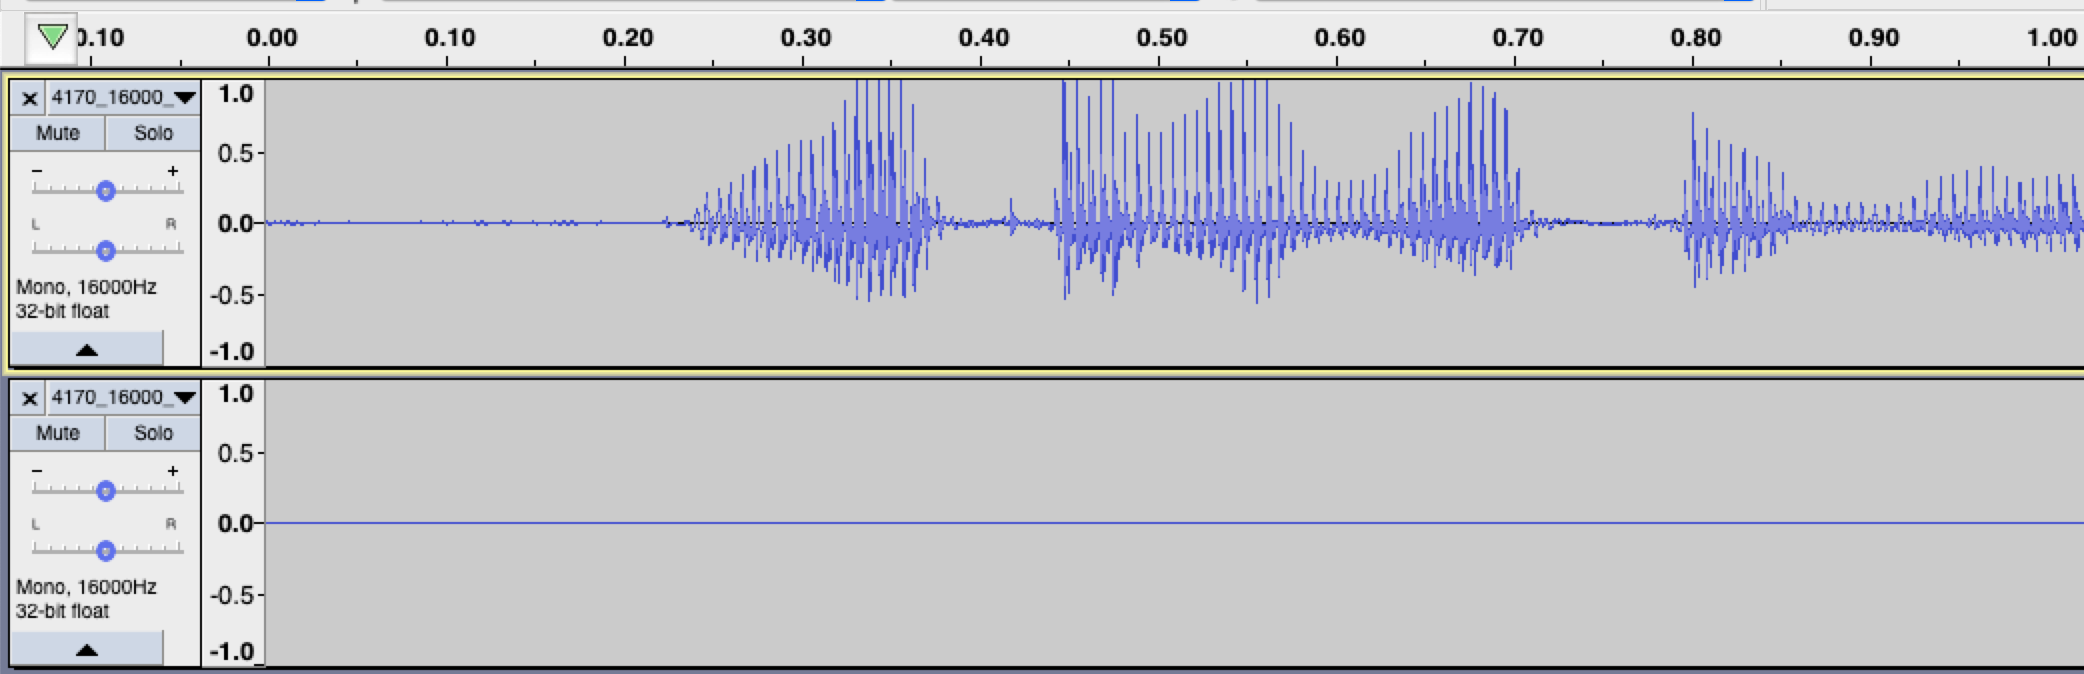
\includegraphics[scale=0.3]{src/main-matter/methodology/preliminary-testing/4170/waveform_4170_1s_chA_top_original}}
	\caption{4170 waveform - The first second of audio - Channel A top, Channel B bottom. Only sound present for Channel A, no sound present for Channel B.}
	\label{fig:upclose_sounding}
\end{figure}
\begin{figure}[h!]
	\centerline{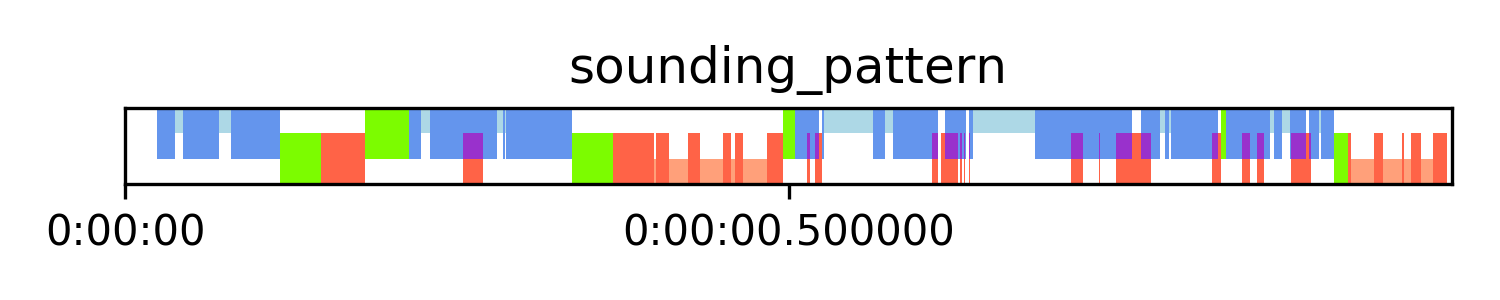
\includegraphics[scale=0.9]{src/main-matter/methodology/preliminary-testing/4170/sounding_pattern_plot_4170_mono_1s_range_short}}
	\caption{4170 Pause Code Plot - The first second of audio - Channel A in blue - Channel B in red. Pause code shows utterances for both channels despite no audio existing for Channel B.}
	\label{fig:upclose_sounding}
\end{figure}

Another example showing pause code producing incorrect results for a five second waveform of the same audio can be seen below. 

\begin{figure}[h!]
	\centerline{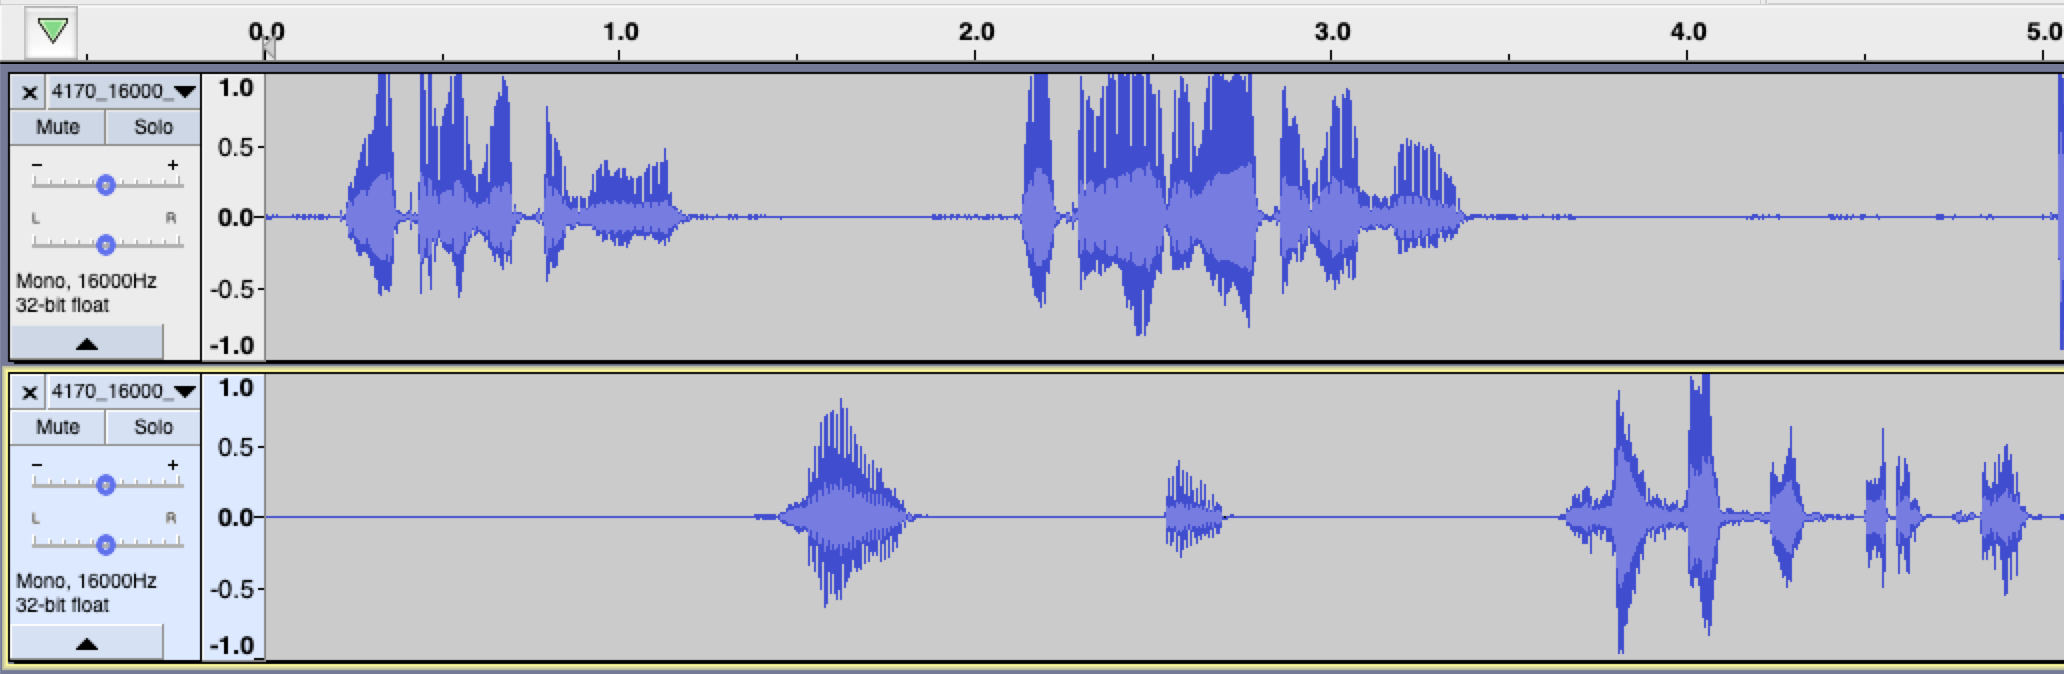
\includegraphics[scale=0.3]{src/main-matter/methodology/preliminary-testing/4170/waveform_4170_5s_chA_top_original}}
	\caption{44170 waveform - The first 5 seconds - Channel A top, Channel B bottom. Only sound present for Channel A, no sound present for Channel B.}
	\label{fig:upclose_sounding}
\end{figure}
\begin{figure}[h!]
	\centerline{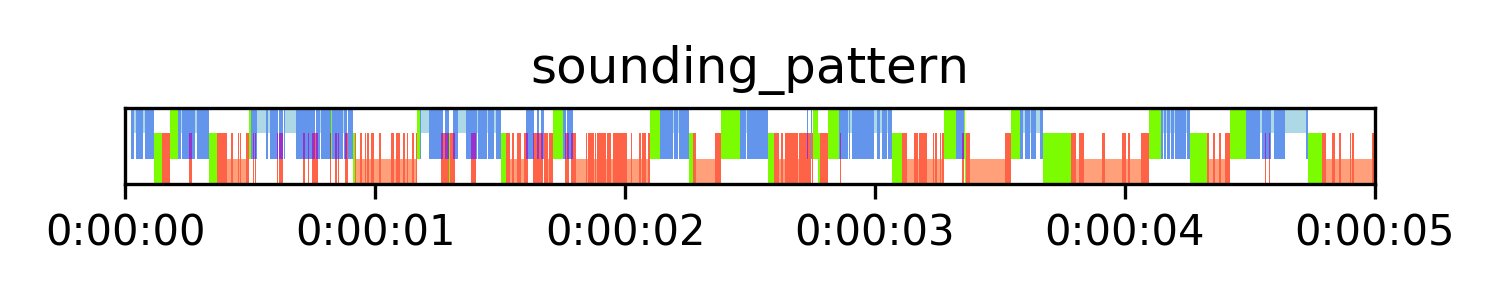
\includegraphics[scale=0.9]{src/main-matter/methodology/preliminary-testing/4170/sounding_pattern_plot_4170_mono_5s_range_short}}
	\caption{4170 Pause Code Plot - The first 5 seconds of audio - Channel A in blue - Channel B in red. Pause code shows more utterances for channel B than what exist in the waveform.}
	\label{fig:upclose_sounding}
\end{figure}



\subsection{Digitisation Process}
A wav file is read in using scipy.io.wavfile, this returns the sampling frequency of the audio file as well as a representation of the audio as an array. This is then sent to the dsp module where the pause and pitch profiles are created. From there the symbolisation process can occur.

\subsection{Digitisation Parameters}
\subsubsection{Time Step}
The Calpy.dsp module digitises the audio. The time\_step controls the level of granularity the audio files is digitised down to be. The smaller the number, the greater the resolution of the binary digitisation. The digitisation was done at the 100ms level, this was a good amount as digitisation returned high resolution results but took roughly 10-20 minutes to do (due to the long lengths of the audio), so decreasing the granularity down any further from the 100ms level would significantly hamper how much data can be retrieved (roughly an hour or two each file). 

\subsubsection{Minimum Silence}
Minimum audio silence is the minimum time required in an audio recording to mark that portion of audio as a silence. 1ms minimum silence was used. 

\subsubsection{Other parameters}
Frame\_window was an extra parameters that controlled the length of speech (in seconds) used to estimate pauses respectively. This was left as is at frame\_window = 0.025. 

\subsubsection{Pause Algorithm} 
This pause algorithm used in Calpy was taken from [Dynamical energy-based speech/silence detector for speech enhancement applications].
%[Sakhnov, K., Verteletskaya, E., \& Simak, B. (2009). Dynamical energy-based speech/silence detector for speech enhancement applications. Proceedings of the World Congress on Engineering (Vol. 1, p. 2).] \\
